%========================================================================================
% TU Dortmund, Informatik Lehrstuhl VII
%========================================================================================

\chapter{Vom Höchstspannungsnetz zum Graphen}
\label{Kapitel 2}
%

\section{Höchstspannungsnetz}
\label{Höchstspannungsnetz}
%
\begin{figure}[t]
	\centering
	{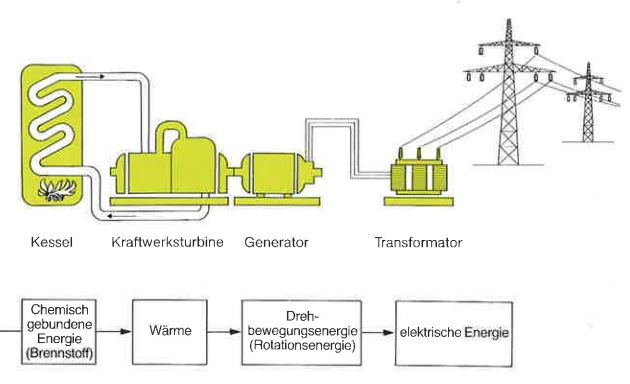
\includegraphics[scale=0.9]{bilder/pds}\label{fig_pds}
	}\\
	\caption[Prinzip der Stromerzeugung]{Prinzip der Stromerzeugung[1]}
	\label{fig_pds}
\end{figure}

\begin{figure}[t]
	\centering
	\subfigure[Niederspannungsleitungen]
	{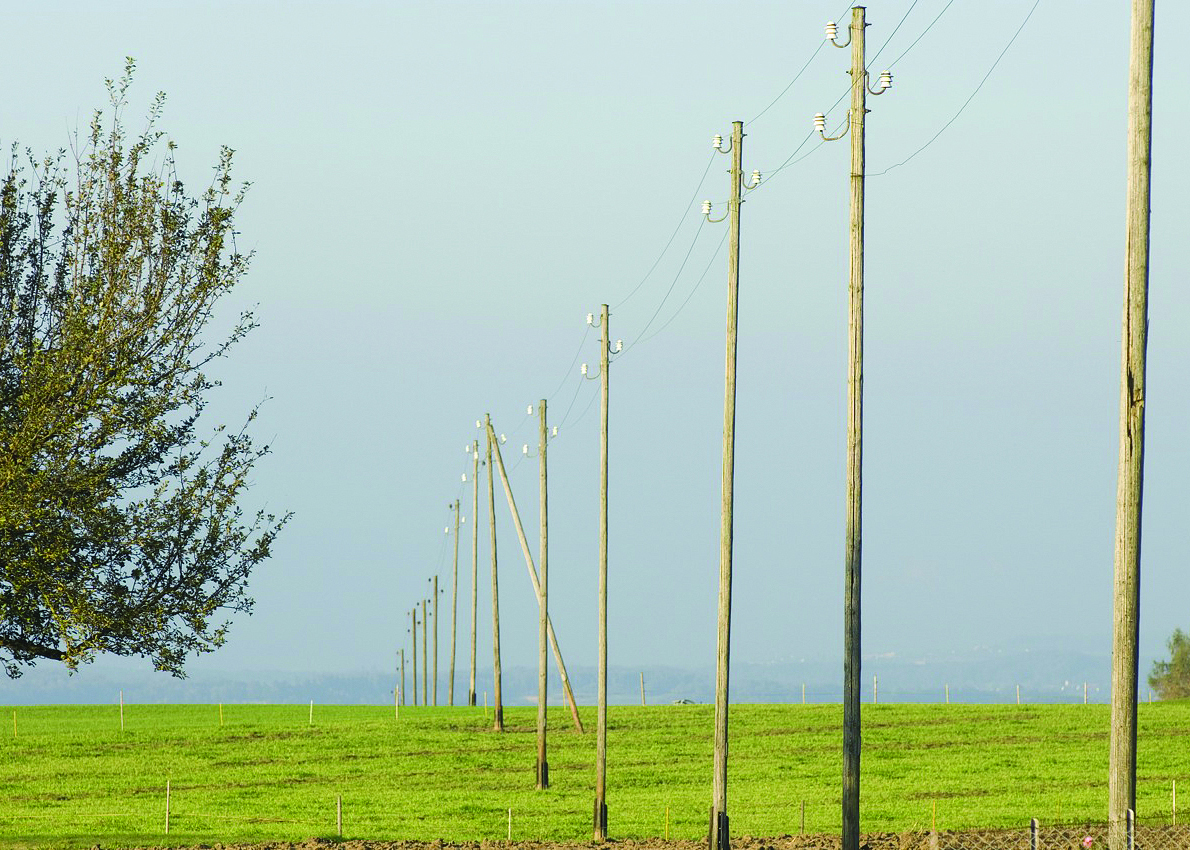
\includegraphics[scale=0.15]{bilder/nieder}\label{fig_nieder}
	}
	\hspace{1.0cm}%
	\subfigure[Mittelspannungsmast]
	{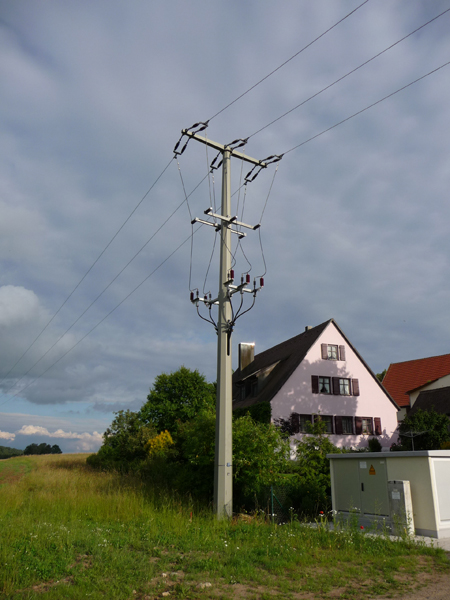
\includegraphics[scale=0.25]{bilder/mittelspannungsleiter}\label{fig_mittelspannungsleiter}
	}
	\hspace{1.0cm}%
	\subfigure[Hochspannungsleitungen]
	{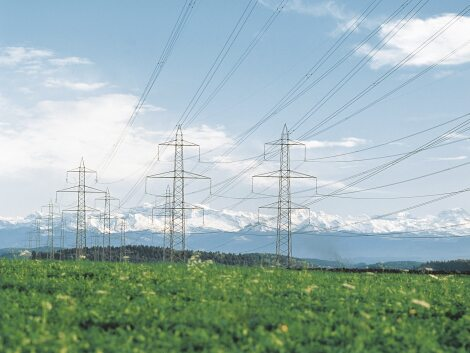
\includegraphics[scale=0.3]{bilder/hochspannungsleitungen}\label{fig_hochspannungsleitungen}
	}
	\hspace{1.0cm}%
	\subfigure[modernisierter Höchstspannungsmast]
	{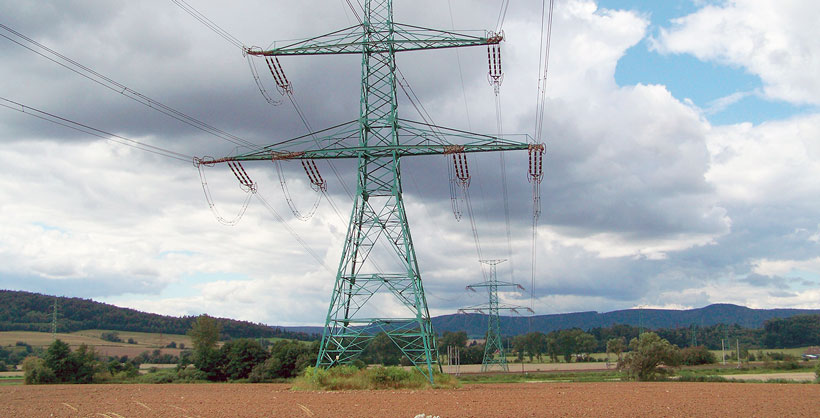
\includegraphics[scale=0.2]{bilder/Reptcheque_HT}\label{fig_Reptcheque_HT}
	}
	\\
	\caption[Die vier verschiedenen Leitungstypen]{Die vier verschiedenen Leitungstypen}
	\label{fig_testbild2}
\end{figure}





\begin{figure}[t]
	\centering
	{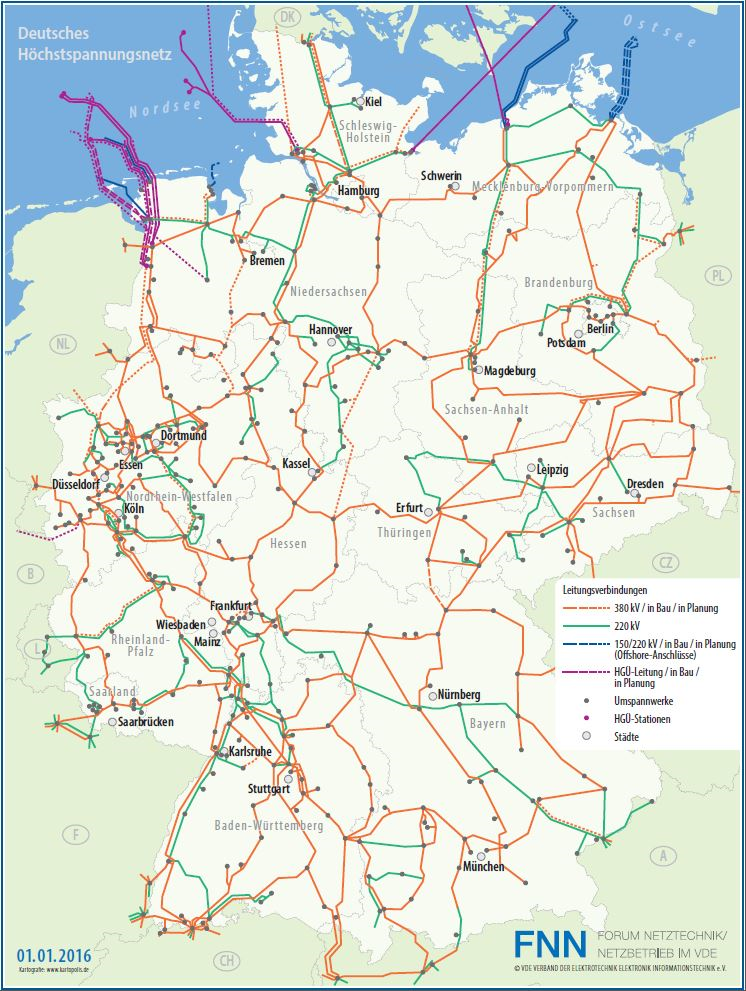
\includegraphics[scale=0.5]{bilder/hochstspannungsnetz}\label{fig_hochstspannungsnetz}
	}\\
	\caption[Karte des deutschen Höchstspannungsnetzes]{Karte des deutschen Höchstspannungsnetzes[1]}
	\label{fig_hochstspannungsnetz2}
\end{figure}
\begin{figure}[t]
	\centering
	{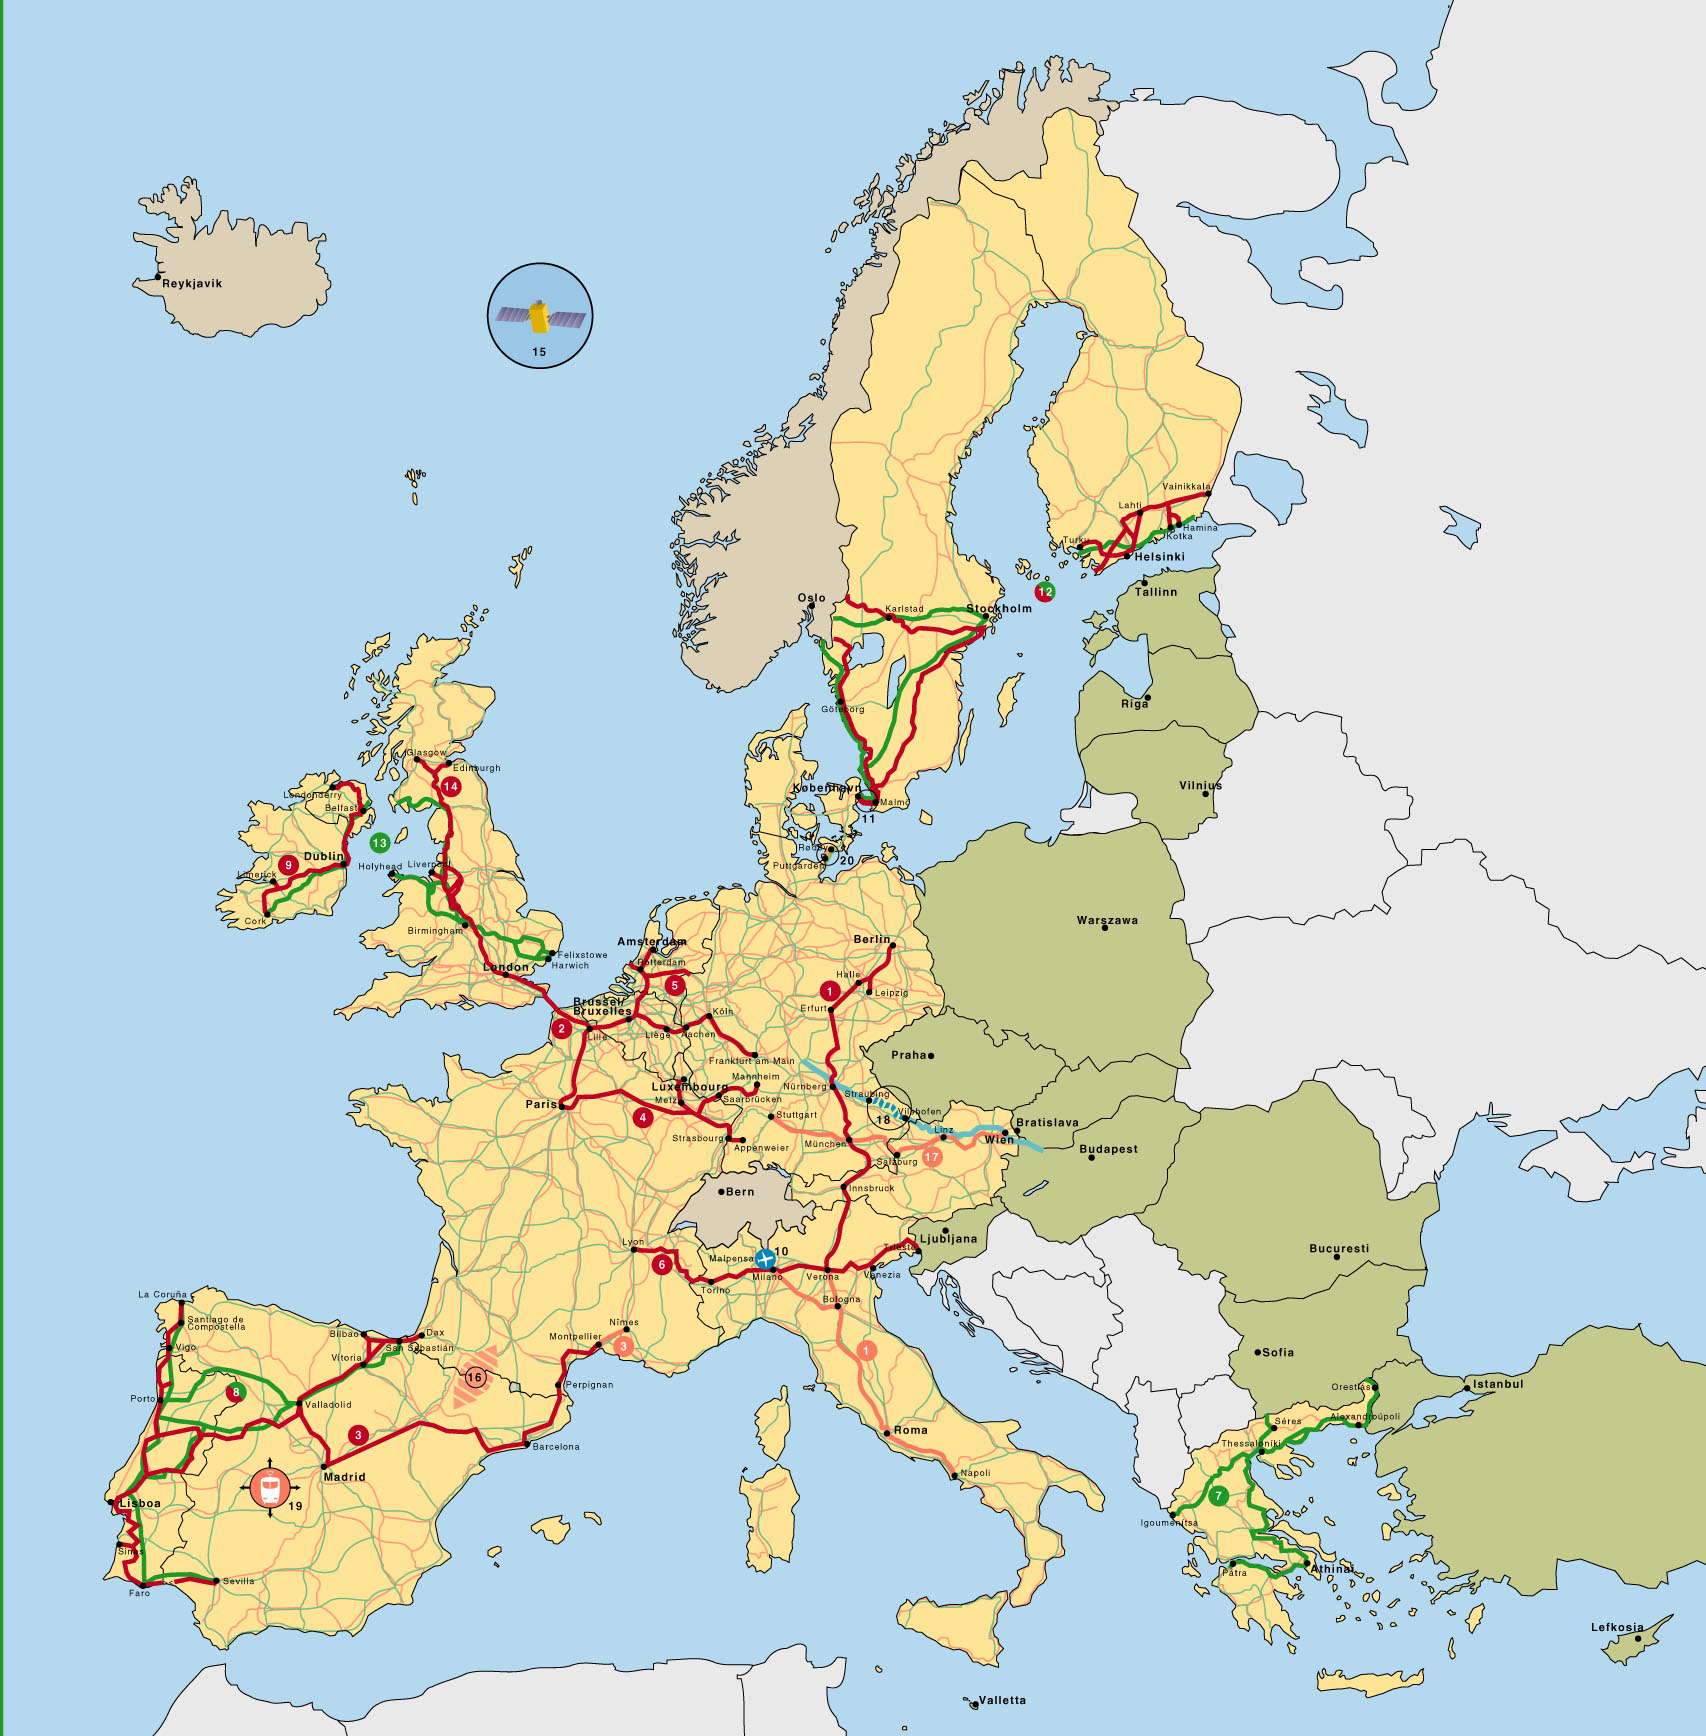
\includegraphics[scale=0.9]{bilder/europastromnetz}\label{fig_europastromnetz}
	}\\
	\caption[Karte des europäischen Verbundnetzes]{Karte des europäischen Verbundnetzes[1]}
	\label{fig_europastromnetz}
\end{figure}

\begin{figure}[t]
	\centering
	{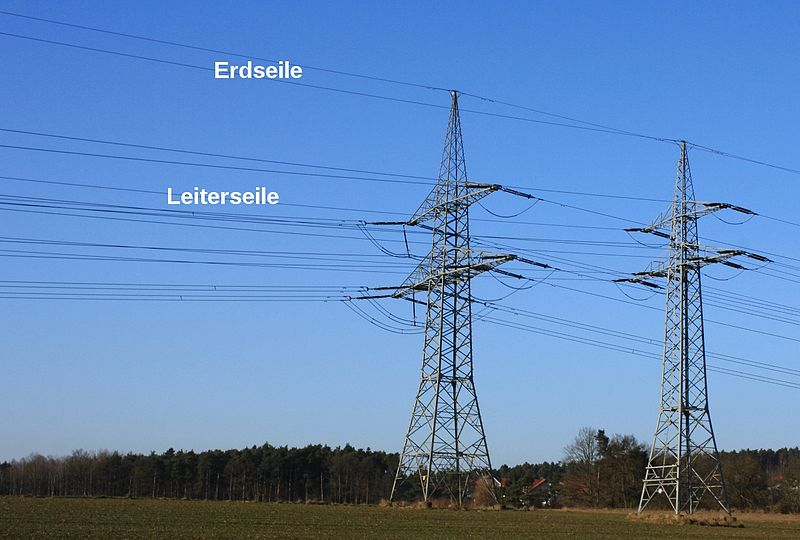
\includegraphics[scale=0.5]{bilder/erdseil}\label{fig_erdseil}
	}\\
	\caption[Freileitungsmast mit Leitern und Erdseil]{Freileitungsmast mit Leitern und Erdseil[1]}
	\label{fig_erdseil}
\end{figure}
Um elektrische Energie über große Distanzen zu transportieren werden Höchstspannungsnetze benutzt. Von einem Kraftwerk ausgehend wird versucht möglichst viele Haushalte, Industrie- und Gewerbebetriebe zu erreichen. Davon ausgehend wird auch der Standort der meisten Kraftwerke bestimmt. Einige Kraftwerke lassen sich nur an bestimmten Standorten errichten, zum Beispiel ein Wasserkraftwerk muss an einem Fluss oder Staudamm errichtet werden. So ist es oft nicht möglich genug Verbraucher zu erreichen, sodass es Mittel bedarf den elektrischen Strom auch über weite Strecken hinweg zu transportieren.

Die Generatoren der modernen Kraftwerke erzeugen eine Spannung von $10500 V$, $21000V$ oder $27000V$[1]. Die Höhe dieser Spannung ist bestimmt durch die Größe bzw. die Leistungsfähigkeit des Kraftwerks und somit von der Nennleistung des Generators.

Da der überwiegende Teil der elektrischen Energie in Wärmekraftwerken erzeugt wird und diese mit einer Generatorleistung von $600$ bis $1300MW$, bedeutet dies, dass Ströme zwischen $15000A$ und $30000A$ abgegeben werden müssen. Das ist jedoch weder aus technischen noch wirtschaftlichen Gründen für einen Transport über lange Distanzen lohnenswert, da es entweder sehr großen Leiterquerschnitte oder sehr große Stromverluste zur Folge hätte.

Es kann die gleiche Leistung $P$ auch mit weniger Strom $I$ und einer erhöhten Spannung $U$ erreicht werden, denn die Beziehung lautet:

\begin{align}
	P = U \cdot I
\end{align}  

Diese Eigenschaft wird ausgenutzt und das führt dazu, dass die Generatorspannung bereits direkt am Kraftwerk durch einen Transformator in eine höhere Spannung umgeformt wird. Dadurch wird die elektrische Leistung mit kleineren Stromstärken über die Netze geleitet. Nur die Übertragung in höheren Spannungen ermöglicht es die elektrische Energie effizient zu übertragen. Die Anpassungen führen zu einem sehr geringen Gesamtverlust von etwa $5\%$ der erzeugten Energie. \\

Die erforderlichen Leitungen um ein effizientes Netz sicherzustellen werden in verschiedenen Ebenen anhand ihrer Betriebsspannung eingeteilt:
\begin{itemize}
	\item Höchstspannungsleitungen mit Betriebsspannungen über $150000V$
	\item Hochspannungsleitungen mit Betriebsspannungen über $60000V$
	\item Mittelspannungsleitungen mit Betriebsspannungen über $1000V$
	\item Niederspannungsleitungen mit Betriebsspannungen bis $1000V$.
\end{itemize} 

In Deutschland werden die Höchstspannungsleitungen mit $380 000V$ oder mit $220 000V$ betrieben. Sie sind zuständig für die überregionale Übertragung. Von den Kraftwerken werden mittels Höchstspannungsleitungen Umspannanlagen, die in der Nähe der Verbraucherschwerpunkte liegen verbunden. In den Umspannanlagen findet eine Herabtransformation auf $110 000V$ statt. Dann sind Hochspannungsleitungen für die weitere regionale Übertragung zuständig. Nach einer weiteren Herabtransformation in einer Umspannanlage beträgt die Spannung noch $10 000V$ oder $20 000V$ und ist jetzt bereit für die Übertragung in der Stadt mittels Mittelspannungsleitungen.

Um die Transportaufgaben zu bewältigen müssen die Höchstspannungsleitungen oft über 100 km lang sein. Das komplette Netz, welches sich über Deutschland erstreckt wird auch das Verbundnetz genannt. Die Einzelnetze werden dabei über Kuppelstellen miteinander verbunden. Das Netz erstreckt sich nicht nur über Deutschland sondern über ganz Europa. Der Vorteil bei einem großen verbundenen Netz sind der Nutz- und Erzeugungsausgleich sowie der kostengünstigen Reservestellung für nicht verbundene Kraftwerke[1].

Da der Stromverbrauch stets variabel ist und sehr örtlich sowie zeitlich unterschiedlich, macht ein großes Verbundnetz viel Sinn. Ebenso aus Sicht der Kraftwerke, zum Beispiel wenn der Schneefall oder Regen ausbleibt, so gibt es an einem Kraftwerk welches an einem Staudamm oder Fluss errichtet worden ist weniger Energie und der Bedarf kann leicht durch andere Quellen über das Netz gedeckt werden.\newline

Es gibt zwei verschiedene Arten für den Transport der elektrischen Energie:
\begin{itemize}
	\item Freileitung
	\item Kabel.
\end{itemize} 
Entschieden wird anhand der technischen Möglichkeiten, die unterschiedlichen physikalischen Eigenschaften der Freileitungen und Kabel, die Kosten sowie Vorstellungen hinsichtlich des Landschaftsschutzes und der Gestaltung des Stadtbildes[1].

Die meisten Leiter bestehen aus Kupfer und Aluminium, dank der hohen Elastizität und elektrischen Leitfähigkeit. Aluminium hat gerade für den Freileitungsbau eine besondere Eigenschaft des sehr geringen Eigengewichtes, was einen größeren Abstand der Masten ermöglicht.

Die Kabel bestehen aus einem Kern der Leiter, welche voneinander durch Isolierungen geschützt werden. Diese nennt man Adern. Mehrere Adern gebunden durch einen Mantel ergeben das letztendliche Kabel, diese können durch ein- oder mehradrig unterschieden werden. Die einzelnen Isolierungen der Adern bestehen aus ölgetränkten Papier, bei niedrigen Spannungen auch Kunststoff(PVC). Die dicke der Isolierung wird durch die jeweilige Nennspannung der Adern bestimmt.

Der Mantel soll die Kabel eng zusammenhalten und gegen äußere mechanische Beschädigungen schützen, ebenso muss er gegen eindringende Feuchtigkeit isolieren. Da Hochspannungsleitungen eine besonders große Isolierung benötigen, werden die Leiter in einem Stahlrohr mit Stickstoffgas unter sehr großen Druck verlegt.

Einzelne Stromkreise und ein Gestänge bilden eine Freileitung. Die Stromkreise bestehen bestehen jeweils aus drei bis vier Leitern. Die spannungsführenden Leiter werden durch Isolatoren an den Masten befestigt, während die anderen Leiter meist durch die Luft isoliert werden. Diese werden auch Seile genannt. 

Es werden verschiedene Werkstoffe zum Bau der Masten verwendet, dabei entscheidet die Größe der Spannung welcher verwendet wird. Diese sind:

\begin{itemize}
	\item Holzmasten für Niederspannungsleitungen 
	\item Holz-/Betonmasten für Mittelspannungsleitungen
	\item Stahlgittermasten für Hoch- und Höchstspannungsleitungen.
\end{itemize} 

Je nachdem wie viel Kraft auf die Masten ausgeübt wird, variiert deren Größe, Konstruktion und Abstand. Äußere Faktoren wie Windbelastungen sowie Schnee- und Eislasten werden dabei mitberücksichtigt.

Die einzelnen Leiter werden mit sogenannten Erdseilen über Isolatoren am jeweiligen Mast angebracht. Die Erdseile dienen dabei nicht dem Transport der elektrischen Energie sondern dem Schutz vor Blitzeinschlägen. Es verlaufen demnach mehrere Stromkreise mit mehreren Leitern und dem Erdseil über einen Mast. In Abbildung 2.5 sieht man die Konstruktion der Masten sehr gut. Ebenso zu sehen sind die jeweiligen Isolatoren zwischen den Leitern und den Masten und das Erdseil welches an der Spitze angebracht ist.

\section{Graph}
\label{Graph}
%


Ein Graph ist ein Tupel $G = (V,E)$ mit folgenden Eigenschaften:

\begin{itemize}
	\item $V$ ist eine nicht leere Menge, die sogenannten Knoten
	\item $E$ ist eine Menge von Kanten zwischen jeweils zwei Knoten[2].
\end{itemize} 

Eine Kante $e_{v_{i},v_{j}} \in E$ mit $v_{i},v_{j} \in V$ repräsentiert somit die Verbindung des Knoten $v_{i}$ mit $v_{j}$.

Ein Graph ist demnach eine Struktur die Informationen anhand Knoten und verbindenden Kanten speichert. Ein einfaches Beispiel sieht man in Abbildung 2.6. Es werden die Städte Köln, Kassel, Frankfurt, Nürnberg und München jeweils durch Knoten repräsentiert und deren Höchstleitungsverbindung durch eine Kante. Es ist nun sehr leicht möglich aus dem Graphen zu entnehmen welche Städte durch Freileitungen miteinander verbunden sind.\\

\begin{figure}[t]
	\centering
	{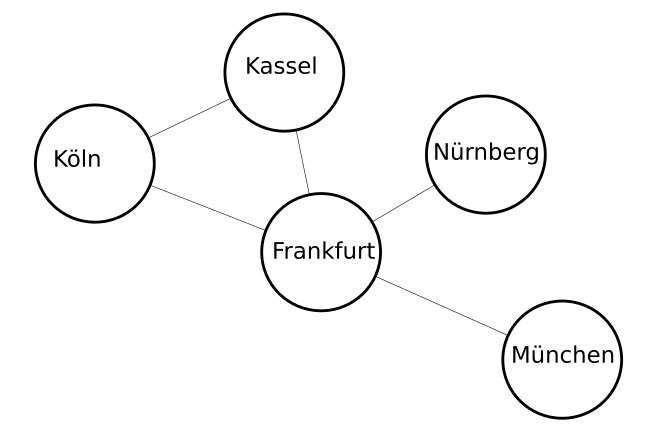
\includegraphics[scale=0.5]{bilder/einfachergraph}\label{fig_einfachergraph}
	}\\
	\caption[Einfacher Graph mit Städten als Knoten und deren Höchstspannungsleitungen als Kanten]{Einfacher Graph mit Städten als Knoten und deren Höchstspannungsleitungen als Kanten}
	\label{fig_einfachergraph}
\end{figure}

Ein Graph kann gerichtet oder ungerichtet sein. Bei einem ungerichteten Graphen gilt: $e_{v_{i},v_{j}} = e_{v_{j},v_{i}}$. Bei einem gerichteten Graphen gilt das nicht immer. Es wird der Kante somit eine Richtung mitgegeben. Ein Knoten $v_{i}$ hat eine Verbindung $e_{v_{i},v_{j}}$ zu einem anderen Knoten $v_{j}$, dies muss jedoch nicht bedeuten dass es auch eine Verbindung ausgehend von $v_{j}$ nach $v_{i}$ gibt. Es werden im Folgenden nur noch ungerichtete Graphen verwendet, somit gilt stets  $e_{v_{i},v_{j}} = e_{v_{j},v_{i}}$.\\

Gibt es keine Kante $e_{v_{i},v_{i}}$ mit $v_{i} \in V$ so ist der Graph schlingenfrei, es existiert also keine Kante von einem Knoten zu sich selbst. Eine Kante heißt demnach Schlinge sofern $e_{v_{i},v_{i}}$ gilt. \\

Kanten sind benachbart oder adjazent, sofern es zwei Knoten $v_{i},v_{j} \in V$ gibt und eine Kante $e_{v_{i},v_{j}} \in E$ sie verbindet. Da nur ungerichtete Graphen verwendet werden, ist es möglich den Start- sowie Endknoten einer Kante stets zu vertauschen und demnach ist auch $e_{v_{j},v_{i}} \in E$ adjazent. \\

Bei einem Graph ist nicht nur die Einhaltung der eigentlichen Struktur wichtig sondern auch wie dessen Knoten und Kanten platziert werden, um eine übersichtliche und anschauliche Zeichnung zu erhalten. Eine wichtige Eigenschaft eines Graphen um dies zu erreichen ist die Planarität. Im Zweidimensionalen Raum ist ein Graph planar sofern es möglich ist diesen so zu zeichnen, dass sich keine Kanten überschneiden. Existiert eine solche Darstellung so ist es auch stets möglich den Graphen planar mit geraden Kanten zu zeichnen[2]. In Abbildung 2.7 ist der Unterschied zwischen dem planaren Graphen und seiner unterschiedlichen Zeichnungen zu sehen. Der planare Graph kann somit auch mit überschneidbaren Kanten gezeichnet werden, mit eckigen oder aber auch immer mit geraden Kanten.


\section{Vom Höchstspannungsnetz zum Graphen}
\label{Vom Höchstspannungsnetz zum Graphen}
%

Es wurden zwei Schritte unternommen um aus dem Höchstspannungsnetz einen repräsentierenden Graphen zu bekommen. Zum einen wurden die jeweiligen Masten zu Knoten und jeweils eins ihrer Leiterseile zu einer verbindenden Kante. Die Position der Masten war aus einer Karte des Höchstspannungsnetz zu bekommen, ebenso deren Verbindungen. 

Da es besonders wichtig ist darzustellen wie viele einzelne Leiterseile über die jeweiligen Verbindungen laufen, musste dieses noch hinzugefügt werden. Es wurde für jedes Leiterseil welches über einen der Masten lief ein jeweiliger Knoten erstellt, und jeweils mit einer Kante verbunden. Diese zusätzlichen Knoten wurden direkt neben dem ursprünglichen Knoten verteilt. Nun hat man die wichtigsten Informationen des Netzes in einen Graphen übertragen.

Die Städte und Orte werden dabei als unbewegliche Knoten angelegt damit der resultierende Graph nicht zu sehr vom ursprünglichen abweicht. Jegliche Eckpunkte zwischen den Orten wurde mithilfe eines weiteren beweglichen Knotens modelliert.

\begin{figure}[t]
	\centering
	\subfigure[Ausschnit des deutschen Höchstspannungsnetzes. Die markierten Orte werden zu den Knoten und die Verbindungen werden zu den Kanten des Graphen.]
	{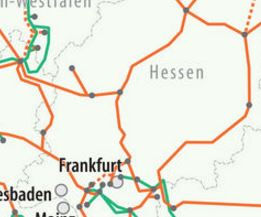
\includegraphics[scale=0.8]{bilder/kartenausschnitt}\label{fig_kartenausschnitt}
	}
	\hspace{1.0cm}%
	\subfigure[Den Ausschnitt der Karte als Graphen mit jeweils nur einer Leitung.]
	{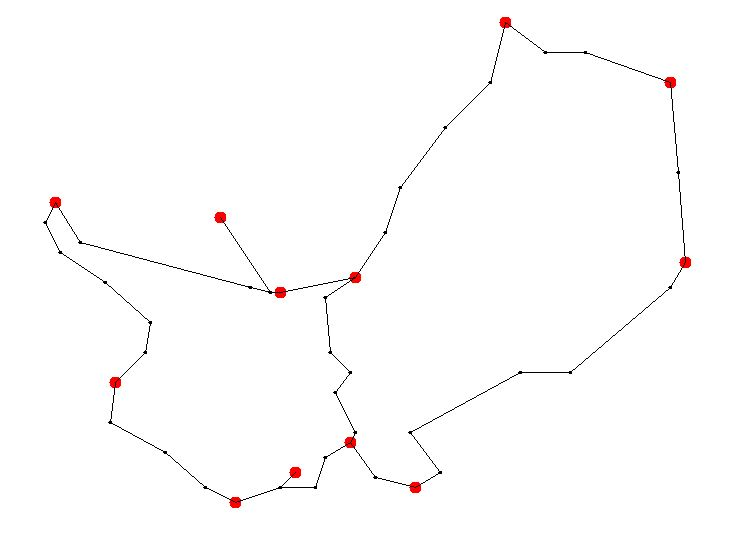
\includegraphics[scale=0.4]{bilder/ausschnittgraph}\label{fig_ausschnittgraph}
	}
	\hspace{1.0cm}%
	\subfigure[Die zusätzlichen Leitungen wurden neben dem eigentlichen Knoten hinzugefügt. Hier jeweils immer genau drei.]
	{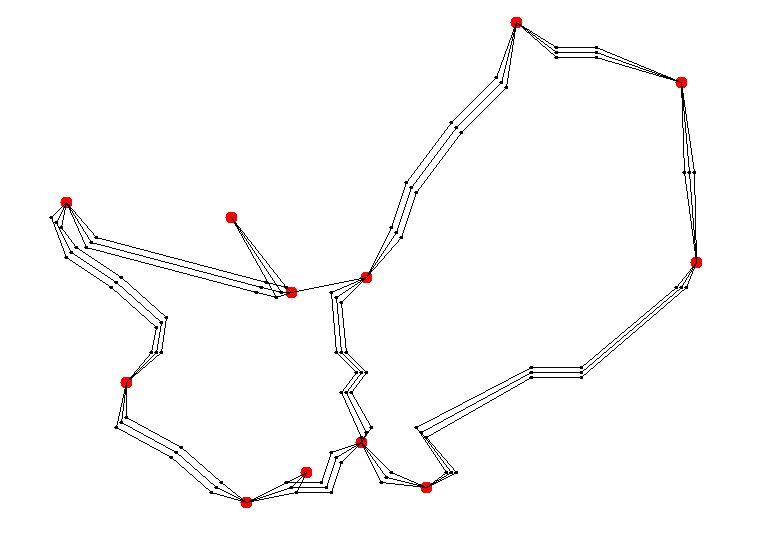
\includegraphics[scale=0.4]{bilder/ausschnittfertigergraph}\label{fig_ausschnittfertigergraph}
	}
	\\
	\caption[Das schrittweise Vorgehen um einen repräsentierenden Graphen zu erhalten]{Das schrittweise Vorgehen um einen repräsentierenden Graphen zu erhalten}
	\label{fig_testbild2}
\end{figure}